
%% bare_conf.tex
%% V1.4
%% 2012/12/27
%% by Michael Shell
%% See:
%% http://www.michaelshell.org/
%% for current contact information.
%%
%% This is a skeleton file demonstrating the use of IEEEtran.cls
%% (requires IEEEtran.cls version 1.8 or later) with an IEEE conference paper.
%%
%% Support sites:
%% http://www.michaelshell.org/tex/ieeetran/
%% http://www.ctan.org/tex-archive/macros/latex/contrib/IEEEtran/
%% and
%% http://www.ieee.org/

%%*************************************************************************
%% Legal Notice:
%% This code is offered as-is without any warranty either expressed or
%% implied; without even the implied warranty of MERCHANTABILITY or
%% FITNESS FOR A PARTICULAR PURPOSE! 
%% User assumes all risk.
%% In no event shall IEEE or any contributor to this code be liable for
%% any damages or losses, including, but not limited to, incidental,
%% consequential, or any other damages, resulting from the use or misuse
%% of any information contained here.
%%
%% All comments are the opinions of their respective authors and are not
%% necessarily endorsed by the IEEE.
%%
%% This work is distributed under the LaTeX Project Public License (LPPL)
%% ( http://www.latex-project.org/ ) version 1.3, and may be freely used,
%% distributed and modified. A copy of the LPPL, version 1.3, is included
%% in the base LaTeX documentation of all distributions of LaTeX released
%% 2003/12/01 or later.
%% Retain all contribution notices and credits.
%% ** Modified files should be clearly indicated as such, including  **
%% ** renaming them and changing author support contact information. **
%%
%% File list of work: IEEEtran.cls, IEEEtran_HOWTO.pdf, bare_adv.tex,
%%                    bare_conf.tex, bare_jrnl.tex, bare_jrnl_compsoc.tex,
%%                    bare_jrnl_transmag.tex
%%*************************************************************************

% *** Authors should verify (and, if needed, correct) their LaTeX system  ***
% *** with the testflow diagnostic prior to trusting their LaTeX platform ***
% *** with production work. IEEE's font choices can trigger bugs that do  ***
% *** not appear when using other class files.                            ***
% The testflow support page is at:
% http://www.michaelshell.org/tex/testflow/



% Note that the a4paper option is mainly intended so that authors in
% countries using A4 can easily print to A4 and see how their papers will
% look in print - the typesetting of the document will not typically be
% affected with changes in paper size (but the bottom and side margins will).
% Use the testflow package mentioned above to verify correct handling of
% both paper sizes by the user's LaTeX system.
%
% Also note that the "draftcls" or "draftclsnofoot", not "draft", option
% should be used if it is desired that the figures are to be displayed in
% draft mode.
%
\documentclass[conference]{IEEEtran}
% Add the compsoc option for Computer Society conferences.
%
% If IEEEtran.cls has not been installed into the LaTeX system files,
% manually specify the path to it like:
% \documentclass[conference]{../sty/IEEEtran}





% Some very useful LaTeX packages include:
% (uncomment the ones you want to load)


% *** MISC UTILITY PACKAGES ***
%
%\usepackage{ifpdf}
% Heiko Oberdiek's ifpdf.sty is very useful if you need conditional
% compilation based on whether the output is pdf or dvi.
% usage:
% \ifpdf
%   % pdf code
% \else
%   % dvi code
% \fi
% The latest version of ifpdf.sty can be obtained from:
% http://www.ctan.org/tex-archive/macros/latex/contrib/oberdiek/
% Also, note that IEEEtran.cls V1.7 and later provides a builtin
% \ifCLASSINFOpdf conditional that works the same way.
% When switching from latex to pdflatex and vice-versa, the compiler may
% have to be run twice to clear warning/error messages.






% *** CITATION PACKAGES ***
%
%\usepackage{cite}
% cite.sty was written by Donald Arseneau
% V1.6 and later of IEEEtran pre-defines the format of the cite.sty package
% \cite{} output to follow that of IEEE. Loading the cite package will
% result in citation numbers being automatically sorted and properly
% "compressed/ranged". e.g., [1], [9], [2], [7], [5], [6] without using
% cite.sty will become [1], [2], [5]--[7], [9] using cite.sty. cite.sty's
% \cite will automatically add leading space, if needed. Use cite.sty's
% noadjust option (cite.sty V3.8 and later) if you want to turn this off
% such as if a citation ever needs to be enclosed in parenthesis.
% cite.sty is already installed on most LaTeX systems. Be sure and use
% version 4.0 (2003-05-27) and later if using hyperref.sty. cite.sty does
% not currently provide for hyperlinked citations.
% The latest version can be obtained at:
% http://www.ctan.org/tex-archive/macros/latex/contrib/cite/
% The documentation is contained in the cite.sty file itself.






% *** GRAPHICS RELATED PACKAGES ***
%
\ifCLASSINFOpdf
  % \usepackage[pdftex]{graphicx}
  % declare the path(s) where your graphic files are
  % \graphicspath{{../pdf/}{../jpeg/}}
  % and their extensions so you won't have to specify these with
  % every instance of \includegraphics
  % \DeclareGraphicsExtensions{.pdf,.jpeg,.png}
\else
  % or other class option (dvipsone, dvipdf, if not using dvips). graphicx
  % will default to the driver specified in the system graphics.cfg if no
  % driver is specified.
  % \usepackage[dvips]{graphicx}
  % declare the path(s) where your graphic files are
  % \graphicspath{{../eps/}}
  % and their extensions so you won't have to specify these with
  % every instance of \includegraphics
  % \DeclareGraphicsExtensions{.eps}
\fi
% graphicx was written by David Carlisle and Sebastian Rahtz. It is
% required if you want graphics, photos, etc. graphicx.sty is already
% installed on most LaTeX systems. The latest version and documentation
% can be obtained at: 
% http://www.ctan.org/tex-archive/macros/latex/required/graphics/
% Another good source of documentation is "Using Imported Graphics in
% LaTeX2e" by Keith Reckdahl which can be found at:
% http://www.ctan.org/tex-archive/info/epslatex/
%
% latex, and pdflatex in dvi mode, support graphics in encapsulated
% postscript (.eps) format. pdflatex in pdf mode supports graphics
% in .pdf, .jpeg, .png and .mps (metapost) formats. Users should ensure
% that all non-photo figures use a vector format (.eps, .pdf, .mps) and
% not a bitmapped formats (.jpeg, .png). IEEE frowns on bitmapped formats
% which can result in "jaggedy"/blurry rendering of lines and letters as
% well as large increases in file sizes.
%
% You can find documentation about the pdfTeX application at:
% http://www.tug.org/applications/pdftex
\usepackage{graphicx}




% *** MATH PACKAGES ***
%
%\usepackage[cmex10]{amsmath}
% A popular package from the American Mathematical Society that provides
% many useful and powerful commands for dealing with mathematics. If using
% it, be sure to load this package with the cmex10 option to ensure that
% only type 1 fonts will utilized at all point sizes. Without this option,
% it is possible that some math symbols, particularly those within
% footnotes, will be rendered in bitmap form which will result in a
% document that can not be IEEE Xplore compliant!
%
% Also, note that the amsmath package sets \interdisplaylinepenalty to 10000
% thus preventing page breaks from occurring within multiline equations. Use:
%\interdisplaylinepenalty=2500
% after loading amsmath to restore such page breaks as IEEEtran.cls normally
% does. amsmath.sty is already installed on most LaTeX systems. The latest
% version and documentation can be obtained at:
% http://www.ctan.org/tex-archive/macros/latex/required/amslatex/math/





% *** SPECIALIZED LIST PACKAGES ***
%
%\usepackage{algorithmic}
% algorithmic.sty was written by Peter Williams and Rogerio Brito.
% This package provides an algorithmic environment fo describing algorithms.
% You can use the algorithmic environment in-text or within a figure
% environment to provide for a floating algorithm. Do NOT use the algorithm
% floating environment provided by algorithm.sty (by the same authors) or
% algorithm2e.sty (by Christophe Fiorio) as IEEE does not use dedicated
% algorithm float types and packages that provide these will not provide
% correct IEEE style captions. The latest version and documentation of
% algorithmic.sty can be obtained at:
% http://www.ctan.org/tex-archive/macros/latex/contrib/algorithms/
% There is also a support site at:
% http://algorithms.berlios.de/index.html
% Also of interest may be the (relatively newer and more customizable)
% algorithmicx.sty package by Szasz Janos:
% http://www.ctan.org/tex-archive/macros/latex/contrib/algorithmicx/




% *** ALIGNMENT PACKAGES ***
%
%\usepackage{array}
% Frank Mittelbach's and David Carlisle's array.sty patches and improves
% the standard LaTeX2e array and tabular environments to provide better
% appearance and additional user controls. As the default LaTeX2e table
% generation code is lacking to the point of almost being broken with
% respect to the quality of the end results, all users are strongly
% advised to use an enhanced (at the very least that provided by array.sty)
% set of table tools. array.sty is already installed on most systems. The
% latest version and documentation can be obtained at:
% http://www.ctan.org/tex-archive/macros/latex/required/tools/


% IEEEtran contains the IEEEeqnarray family of commands that can be used to
% generate multiline equations as well as matrices, tables, etc., of high
% quality.




% *** SUBFIGURE PACKAGES ***
%\ifCLASSOPTIONcompsoc
%  \usepackage[caption=false,font=normalsize,labelfont=sf,textfont=sf]{subfig}
%\else
%  \usepackage[caption=false,font=footnotesize]{subfig}
%\fi
% subfig.sty, written by Steven Douglas Cochran, is the modern replacement
% for subfigure.sty, the latter of which is no longer maintained and is
% incompatible with some LaTeX packages including fixltx2e. However,
% subfig.sty requires and automatically loads Axel Sommerfeldt's caption.sty
% which will override IEEEtran.cls' handling of captions and this will result
% in non-IEEE style figure/table captions. To prevent this problem, be sure
% and invoke subfig.sty's "caption=false" package option (available since
% subfig.sty version 1.3, 2005/06/28) as this is will preserve IEEEtran.cls
% handling of captions.
% Note that the Computer Society format requires a larger sans serif font
% than the serif footnote size font used in traditional IEEE formatting
% and thus the need to invoke different subfig.sty package options depending
% on whether compsoc mode has been enabled.
%
% The latest version and documentation of subfig.sty can be obtained at:
% http://www.ctan.org/tex-archive/macros/latex/contrib/subfig/




% *** FLOAT PACKAGES ***
%
%\usepackage{fixltx2e}
% fixltx2e, the successor to the earlier fix2col.sty, was written by
% Frank Mittelbach and David Carlisle. This package corrects a few problems
% in the LaTeX2e kernel, the most notable of which is that in current
% LaTeX2e releases, the ordering of single and double column floats is not
% guaranteed to be preserved. Thus, an unpatched LaTeX2e can allow a
% single column figure to be placed prior to an earlier double column
% figure. The latest version and documentation can be found at:
% http://www.ctan.org/tex-archive/macros/latex/base/


%\usepackage{stfloats}
% stfloats.sty was written by Sigitas Tolusis. This package gives LaTeX2e
% the ability to do double column floats at the bottom of the page as well
% as the top. (e.g., "\begin{figure*}[!b]" is not normally possible in
% LaTeX2e). It also provides a command:
%\fnbelowfloat
% to enable the placement of footnotes below bottom floats (the standard
% LaTeX2e kernel puts them above bottom floats). This is an invasive package
% which rewrites many portions of the LaTeX2e float routines. It may not work
% with other packages that modify the LaTeX2e float routines. The latest
% version and documentation can be obtained at:
% http://www.ctan.org/tex-archive/macros/latex/contrib/sttools/
% Do not use the stfloats baselinefloat ability as IEEE does not allow
% \baselineskip to stretch. Authors submitting work to the IEEE should note
% that IEEE rarely uses double column equations and that authors should try
% to avoid such use. Do not be tempted to use the cuted.sty or midfloat.sty
% packages (also by Sigitas Tolusis) as IEEE does not format its papers in
% such ways.
% Do not attempt to use stfloats with fixltx2e as they are incompatible.
% Instead, use Morten Hogholm'a dblfloatfix which combines the features
% of both fixltx2e and stfloats:
%
% \usepackage{dblfloatfix}
% The latest version can be found at:
% http://www.ctan.org/tex-archive/macros/latex/contrib/dblfloatfix/




% *** PDF, URL AND HYPERLINK PACKAGES ***
%
%\usepackage{url}
% url.sty was written by Donald Arseneau. It provides better support for
% handling and breaking URLs. url.sty is already installed on most LaTeX
% systems. The latest version and documentation can be obtained at:
% http://www.ctan.org/tex-archive/macros/latex/contrib/url/
% Basically, \url{my_url_here}.




% *** Do not adjust lengths that control margins, column widths, etc. ***
% *** Do not use packages that alter fonts (such as pslatex).         ***
% There should be no need to do such things with IEEEtran.cls V1.6 and later.
% (Unless specifically asked to do so by the journal or conference you plan
% to submit to, of course. )


% correct bad hyphenation here
\hyphenation{op-tical net-works semi-conduc-tor}


\begin{document}
%
% paper title
% can use linebreaks \\ within to get better formatting as desired
% Do not put math or special symbols in the title.
\title{Projeto 1}


% author names and affiliations
% use a multiple column layout for up to three different
% affiliations
\author{\IEEEauthorblockN{Gustavo Antonio Souza de Barros}
\IEEEauthorblockA{18/0064487\\Introdução ao processamento de imagens\\Engenharia da Computação\\
Universidade de Brasília\\
Brasília, Distrito Federal 70910-900\\
Email: gustavoasb@gmail.com}
}

% conference papers do not typically use \thanks and this command
% is locked out in conference mode. If really needed, such as for
% the acknowledgment of grants, issue a \IEEEoverridecommandlockouts
% after \documentclass

% for over three affiliations, or if they all won't fit within the width
% of the page, use this alternative format:
% 
%\author{\IEEEauthorblockN{Michael Shell\IEEEauthorrefmark{1},
%Homer Simpson\IEEEauthorrefmark{2},
%James Kirk\IEEEauthorrefmark{3}, 
%Montgomery Scott\IEEEauthorrefmark{3} and
%Eldon Tyrell\IEEEauthorrefmark{4}}
%\IEEEauthorblockA{\IEEEauthorrefmark{1}School of Electrical and Computer Engineering\\
%Georgia Institute of Technology,
%Atlanta, Georgia 30332--0250\\ Email: see http://www.michaelshell.org/contact.html}
%\IEEEauthorblockA{\IEEEauthorrefmark{2}Twentieth Century Fox, Springfield, USA\\
%Email: homer@thesimpsons.com}
%\IEEEauthorblockA{\IEEEauthorrefmark{3}Starfleet Academy, San Francisco, California 96678-2391\\
%Telephone: (800) 555--1212, Fax: (888) 555--1212}
%\IEEEauthorblockA{\IEEEauthorrefmark{4}Tyrell Inc., 123 Replicant Street, Los Angeles, California 90210--4321}}




% use for special paper notices
%\IEEEspecialpapernotice{(Invited Paper)}




% make the title area
\maketitle

% As a general rule, do not put math, special symbols or citations
% in the abstract
\begin{abstract}
O projeto desenvolvido tem como objetivo a realização de duas atividades.
A primeira tem foco na manipulação de imagens, criando uma função que mude a
quantidade de bits da imagem, assim como seu tamanho. A segunda aborda sobre
um problema dado, em que um conjunto de astronautas tem de obter uma amostra de 
solo de um local específico de Marte. Através de uma imagem aérea RGB, o objetivo
é achar o jeito mais rápido de chegar a esse local usando a menor energia possível.
\end{abstract}

% no keywords




% For peer review papers, you can put extra information on the cover
% page as needed:
% \ifCLASSOPTIONpeerreview
% \begin{center} \bfseries EDICS Category: 3-BBND \end{center}
% \fi
%
% For peerreview papers, this IEEEtran command inserts a page break and
% creates the second title. It will be ignored for other modes.
\IEEEpeerreviewmaketitle



\section{Introduction}
% no \IEEEPARstart
O processamento de imagens é um tópico que está sempre em pauta quando se
trata de novas tecnologias. O crescimento dessa área é exponencial e compreende
diversas aplicações. 

A capacidade de manejar imagens a fim de adquirir dados ou implementar funcionalidades
é extretamente importante, tornando o projeto essencial para o treinamento
desta capacitações.

A fim de entender melhor a finalidade da primeira tarefa, é necessário
ter conhecimento sobre o que são os bits quando se fala de imagem. Um bit é o que chamamos
de profundidade de cor, de um jeito simplificado, descreve a quantidade de 
cores que os pixels da imagem podem ser representados. Através da equação abaixo
é facil perceber como isso se aplica.

\begin{equation}\label{eq1}
    Cores = 2^n
\end{equation}

Na equação 1 ,  \textit{n} representa o número de bits, logo podemos montar o esquema abaixo:

\begin{itemize}
\item 1 bit, $2^1$ = 2 cores, imagem binária.
\item 2 bit, $2^2$ = 4 cores.
\item 3 bit, $2^3$ = 8 cores.
\item 4 bit, $2^4$ = 16 cores.
\item 5 bit, $2^5$ = 32 cores.
\item 6 bit, $2^6$ = 64 cores.
\item 7 bit, $2^7$ = 128 cores.
\item 8 bit, $2^8$ = 256 cores.
\end{itemize}

Em imagens não coloridas, nós assumimos que os pixels tem 
o que chamamos de intensidade, que se refere ao brilho do mesmo.
Um pixel com brilho 255 em uma imagem com 256 bits é branco, e um com 0
é preto. Entre esses vários pixels estão os tons de cinza, que são determinados
pela quantidade de bits da imagem.

Em imagens coloridas, nós entramos no tópico do RGB (Red, Green, Blue), que
são como as cores de uma imagem são apresentadas. Cada cor tem uma quantidade
de cada um desses componentes e assim podemos representa-las com valores destes.
Para esse tipo de imagem, a quantidade de bits se refere a quantidade maxima que
cada componente pode chegar.

\section{Metodologia}
% no \IEEEPARstart
\subsection{Questão 1}

Para a primeira atividade, foram desenvolvidas rotinas que alteram a quantidade
de bits de uma imagem, assim como suas dimensões. O código fonte está salvo
como question1.py e pode ser executado através da linha de comando \textit{python question1.py}.


Primeiramente, lê se a imagem teste, com auxílio do OpenCV. Após isso, foi implementada
uma função que muda a quantidade de bits da imagem através da entrada do usuário,
através de uma fórmula matemática que faz isso automaticamente.

\begin{equation}
    \label{eq2}
    \frac{pixel value}{256/2^n}
\end{equation}

Sendo \textit{n} a quantidade de bits desejada.

Após a conversão realiza-se arredondamentos e adapta-se a imagem de volta
para a quantidade de bits padrão, 256. Esse procedimento é adotado pois
o foco é apenas demonstrar a diferença entre as imagens de bits diferentes, 
e não converte-las em si.

A segunda parte dessa atividade é baseado no redimensionamento de uma imagem,
o usuário dará um valor que definirá as novas dimensões da mesma.

\begin{equation}
    H_{nova} = H_{original} \cdot k
\end{equation}
\begin{equation}
    L_{nova} = L_{original} \cdot k
\end{equation}

Sendo \textit{k} o valor que definido para mudar o tamanho da imagem. 
Por exemplo, k = 0.5 retornaria uma imagem com metade do tamanho original.

Para k menor que 1, pode-se simplesmente repetir os pixels da original
de forma a jogar alguns valores fora. 
Porém para valores elevados de k nós deparamos com o problema de espaços vazios.
Para resolver isso repete-se a última linha lida e coloca-se no espaço vazio encontrado.
O mesmo procedimento é efetuado para colunas, fechando assim a imagem redimensionada.

\subsection{Questão 2}

Para a segunda atividade, lê-se o mapa aéreo de marte com cores RGB com intensidades
a indicar a energia gastada para passar naquele local. Tira-se dali um caminho curto e com
gasto de energia mais baixo possível.

O primeiro procedimento adotado é converter a imagem de RGB para monocromática. Isso é facilmente
resolvido usando a fórmula:

\begin{equation}
    \label{eq5}
    Intensitidade = \frac{R+G+B}{3}
\end{equation}

Realizando a rotina para todos os pixels consegue-se uma imagem em tons
de cinza. 

Após isso, com ajuda do OpenCV realiza-se a equalização do histograma da imagem,
a fim de enaltecer os detalhes, através do aumento do contraste.

Com origem e destino definidos, inicia-se um loop que altera o pixel em que o algoritmo
está atualmente localizado, e que será finalizado quando é alcançado o pixel de destino.

O laço anteriormente citado funciona da seguinte maneira, os 8 pixeis ao redor do atualmente
são os candidatos a serem escolhidos como próximo do caminho. Mas para isso existem condições,
primeiro efetua-se a distância euclediana entre os 8 e o pixel de destino, através da equação:

\begin{equation}
    \label{eq6}
    Distancia = \sqrt{(x - x_{f})^2 + (y - y_{f})^2}
\end{equation}

Depois dos cálculos, efetua-se uma ordenação pela distância e as três menores vão
para a próxima etapa.

Com os pixels de menor distância ajustados, faz-se um teste com estes e é selecionado
o de menor intensidade. Esse selecionado é o novo pixel que irá compor o caminho até 
a localização final, e a partir dele a fase de seleção iniciará de novo, processo que se repete
inúmeras vezes, de forma a alcançar o local almejado.
% An example of a floating figure using the graphicx package.
% Note that \label must occur AFTER (or within) \caption.
% For figures, \caption should occur after the \incWludegraphics.
% Note that IEEEtran v1.7 and later has special internal code that
% is designed to preserve the operation of \label within \caption
% even when the captionsoff option is in effect. However, because
% of issues like this, it may be the safest practice to put all your
% \label just after \caption rather than within \caption{}.
%
% Reminder: the "draftcls" or "draftclsnofoot", not "draft", class
% option should be used if it is desired that the figures are to be
% displayed while in draft mode.
%
%\begin{figure}[!t]
%\centering
%\includegraphics[width=2.5in]{myfigure}
% where an .eps filename suffix will be assumed under latex, 
% and a .pdf suffix will be assumed for pdflatex; or what has been declared
% via \DeclareGraphicsExtensions.
%\caption{Simulation Results.}
%\label{fig_sim}
%\end{figure}

% Note that IEEE typically puts floats only at the top, even when this
% results in a large percentage of a column being occupied by floats.


% An example of a double column floating figure using two subfigures.
% (The subfig.sty package must be loaded for this to work.)
% The subfigure \label commands are set within each subfloat command,
% and the \label for the overall figure must come after \caption.
% \hfil is used as a separator to get equal spacing.
% Watch out that the combined width of all the subfigures on a 
% line do not exceed the text width or a line break will occur.
%
%\begin{figure*}[!t]
%\centering
%\subfloat[Case I]{\includegraphics[width=2.5in]{box}%
%\label{fig_first_case}}
%\hfil
%\subfloat[Case II]{\includegraphics[width=2.5in]{box}%
%\label{fig_second_case}}
%\caption{Simulation results.}
%\label{fig_sim}
%\end{figure*}
%
% Note that often IEEE papers with subfigures do not employ subfigure
% captions (using the optional argument to \subfloat[]), but instead will
% reference/describe all of them (a), (b), etc., within the main caption.


% An example of a floating table. Note that, for IEEE style tables, the 
% \caption command should come BEFORE the table. Table text will default to
% \footnotesize as IEEE normally uses this smaller font for tables.
% The \label must come after \caption as always.
%
%\begin{table}[!t]
%% increase table row spacing, adjust to taste
%\renewcommand{\arraystretch}{1.3}
% if using array.sty, it might be a good idea to tweak the value of
% \extrarowheight as needed to properly center the text within the cells
%\caption{An Example of a Table}
%\label{table_example}
%\centering
%% Some packages, such as MDW tools, offer better commands for making tables
%% than the plain LaTeX2e tabular which is used here.
%\begin{tabular}{|c||c|}
%\hline
%One & Two\\
%\hline
%Three & Four\\
%\hline
%\end{tabular}
%\end{table}


% Note that IEEE does not put floats in the very first column - or typically
% anywhere on the first page for that matter. Also, in-text middle ("here")
% positioning is not used. Most IEEE journals/conferences use top floats
% exclusively. Note that, LaTeX2e, unlike IEEE journals/conferences, places
% footnotes above bottom floats. This can be corrected via the \fnbelowfloat
% command of the stfloats package.

\section{Resultados}

Essa seção abordará sobre os resultados encontrados nos tópicos debatidos
anteriormente.

\subsection{Questão 1}

A imagem original dos testes é mostrada abaixo para efeito comparativo.

\begin{figure}[h]
    \centering
    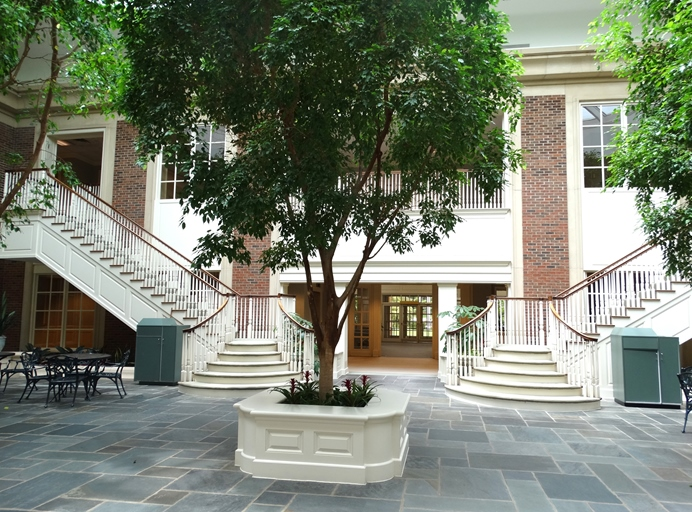
\includegraphics[scale=0.3]{im1.jpg}
    \caption{Imagem original}
    \label{fig1}
\end{figure}

O primeiro teste da atividade inicial é com um valor de redimensionamento
menor que 1. Para ele as entradas foram (5,0.5):

\begin{figure}[h]
    \centering
    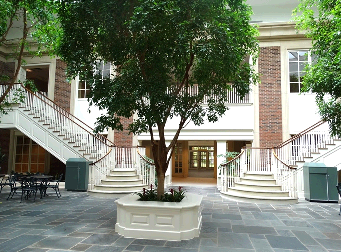
\includegraphics[scale=0.7]{Figs/saida1.png}
    \caption{Saída 1}
    \label{fig1}
\end{figure}

A diferença entre a original e a do primeira teste é mínima, pois
trata-se de diminuição a diferença de bits não é tão chamativa.

O segundo teste foi efetuado usando as entradas (3,1.75):
\begin{figure}[h]
    \centering
    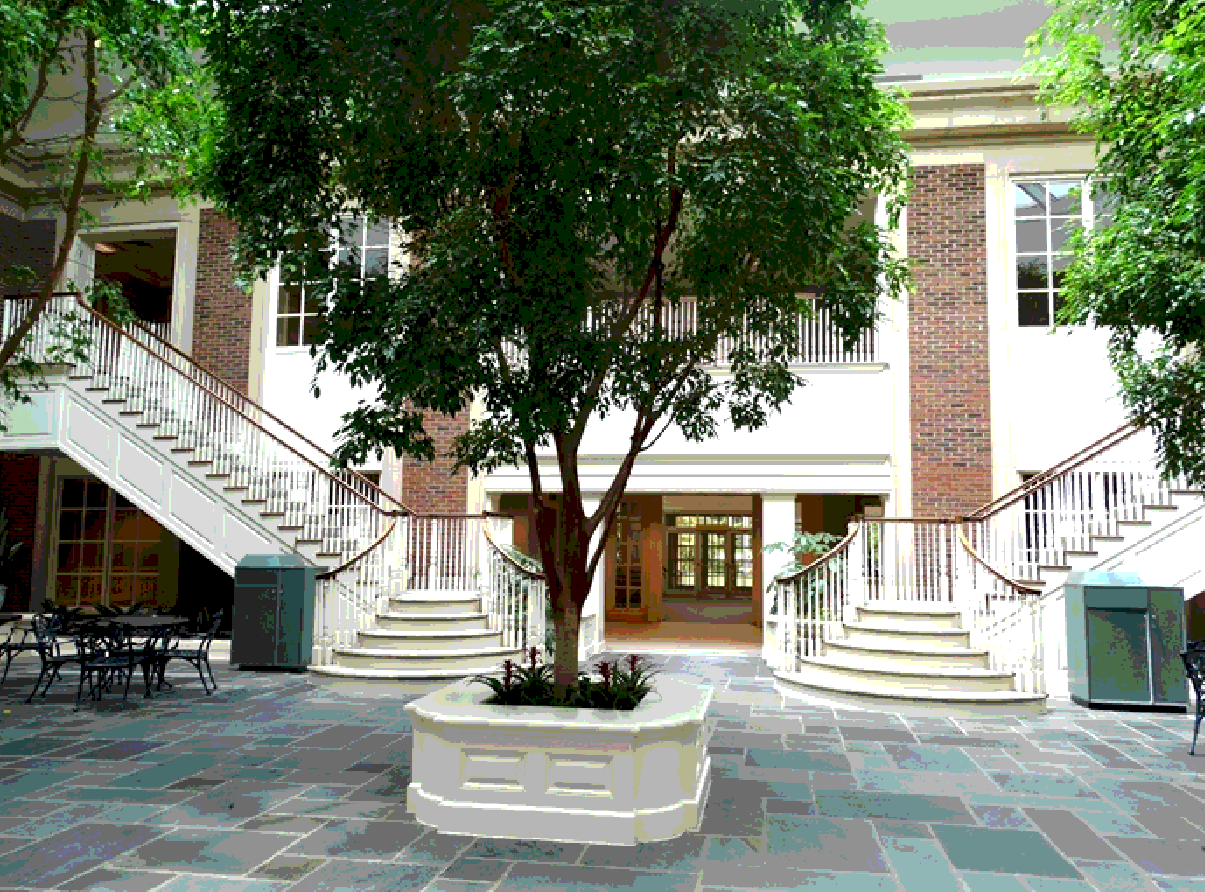
\includegraphics[scale=0.20]{Figs/saida2.png}
    \caption{Saída 2}
    \label{fig2}
\end{figure}

No teste 2 já é possível notar a diferença nas cores, que perdem detalhe,
e se aberta a imagem original seria mais clara a perda de qualidade
da imagem ao ser aumentada.

Para um última checagem, testa-se um imagem em tons de cinza. As entradas
foram (2,1)

\begin{figure}[h]
    \centering
    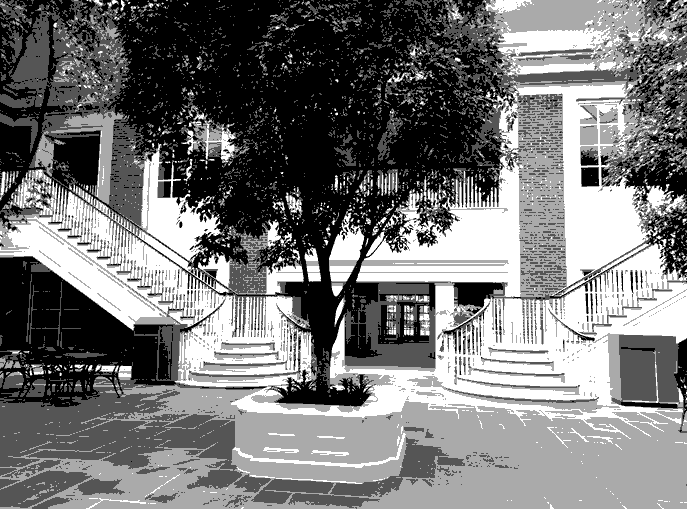
\includegraphics[scale=0.35]{Figs/saida3.png}
    \caption{Saída 3}
    \label{fig2}
\end{figure}

é evidente a transformação das cores ao usarmos apenas 2 bits. A imagem não
foi redimensionada pelo coeficiente ser 1.

\subsection{Questão 2}

\begin{figure}[h]
    \centering
    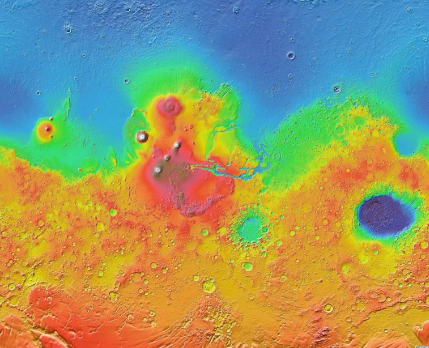
\includegraphics[scale=0.6]{Figs/mars.png}
    \caption{Mapa aéreo de Marte, Questão 2}
    \label{fig2}
\end{figure}

Através do mapa aéreo acima, acha-se o caminho usando o algoritmo explicado
anteriormente, tendo como saída:

\begin{figure}[h]
    \centering
    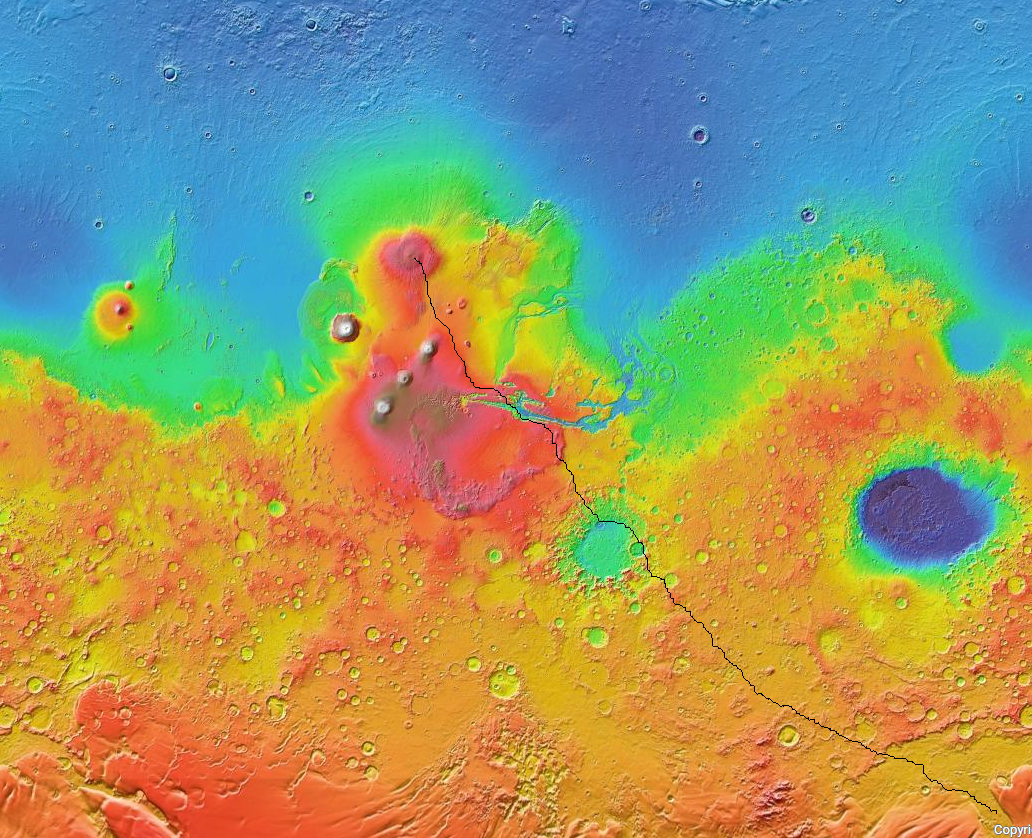
\includegraphics[scale=0.25]{Figs/path.png}
    \caption{Saída, Questão 2}
    \label{fig2}
\end{figure}

O caminho marcado em preto foi o encontrado como o balanço entre distância
e gasto de energia.

\section{Conclusões}

Levando em conta toda a realização do projeto, considera-se que este foi 
executado com sucesso e com resultados aceitáveis. Apesar de ter sido concluído
de forma decente, há espaço para melhores, existem algoritmos de redimensionamento
extremamente superiores, além de execuções que poderiam ser muito mais rápidas
se fossem trabalhadas de forma mais minuciosa.

Os resultados deram a perceber na prática como funcionam diversos dos conceitos
desenvolvidos em sala de aula, além de uma maior percepção do assunto.

Assuntos como o aumento ou diminuição de imagens de forma a deixar a imagem
de forma mais agradável possível fora um assunto interessante, pois faz-se constestar
como funcionam os melhores algoritmos para essas rotinas.





% conference papers do not normally have an appendix






% trigger a \newpage just before the given reference
% number - used to balance the columns on the last page
% adjust value as needed - may need to be readjusted if
% the document is modified later
%\IEEEtriggeratref{8}
% The "triggered" command can be changed if desired:
%\IEEEtriggercmd{\enlargethispage{-5in}}

% references section

% can use a bibliography generated by BibTeX as a .bbl file
% BibTeX documentation can be easily obtained at:
% http://www.ctan.org/tex-archive/biblio/bibtex/contrib/doc/
% The IEEEtran BibTeX style support page is at:
% http://www.michaelshell.org/tex/ieeetran/bibtex/
%\bibliographystyle{IEEEtran}
% argument is your BibTeX string definitions and bibliography database(s)
%\bibliography{IEEEabrv,../bib/paper}
%
% <OR> manually copy in the resultant .bbl file
% set second argument of \begin to the number of references
% (used to reserve space for the reference number labels box)
\begin{thebibliography}{1}

\bibitem{OpenCV}
OpenCV Team, \emph{Open Source Computer Vision Documentation}.\hskip 1em plus
  0.5em minus 0.4em\relax opencv.org.

\bibitem{Colord}
Wikipedia, \emph{Color depth}.\hskip 1em plus
  0.5em minus 0.4em\relax Acessed in 20, April, 2019.

\bibitem{SciPy}
SciPy Team, \emph{NumPy User Guide}.\hskip 1em plus
  0.5em minus 0.4em\relax docs.scipy.org.

\bibitem{Pbarret}
Paul Barrett, \emph{Euclidean Distance},\hskip 1em plus
  0.5em minus 0.4em\relax September, 2015, www.pbarrett.net/techpapers/euclid.pdf.

  \bibitem{SciPy}
  Gerald Bakker, \emph{Color Coding and the RGB Color Space},\hskip 1em plus
  0.5em minus 0.4em\relax December, 2014, geraldbakker.nl/psnumbers/rgb-explained.html.

\end{thebibliography}




% that's all folks
\end{document}


